\chapter{Renderer experiments from bijou-fun}\label{renderer-gallery}

These two captures come from the separate \texttt{bijou-fun} demonstration application. Its registry contains gradients, a wormhole, fluid simulations, raymarching, a raycaster, font rendering, a text cylinder, metaballs and a raytracer. The inspected checkout was \texttt{0685ddc993491d309468b4f3ca7bc5e6a6e5f4b0}; its installed Bijou package was 7.1.0. The source modules were called directly with a controlled viewport and input values; the network checkout was left unchanged.

\section{Raymarching in terminal cells}
\subsection{Lighting becomes glyph and color}

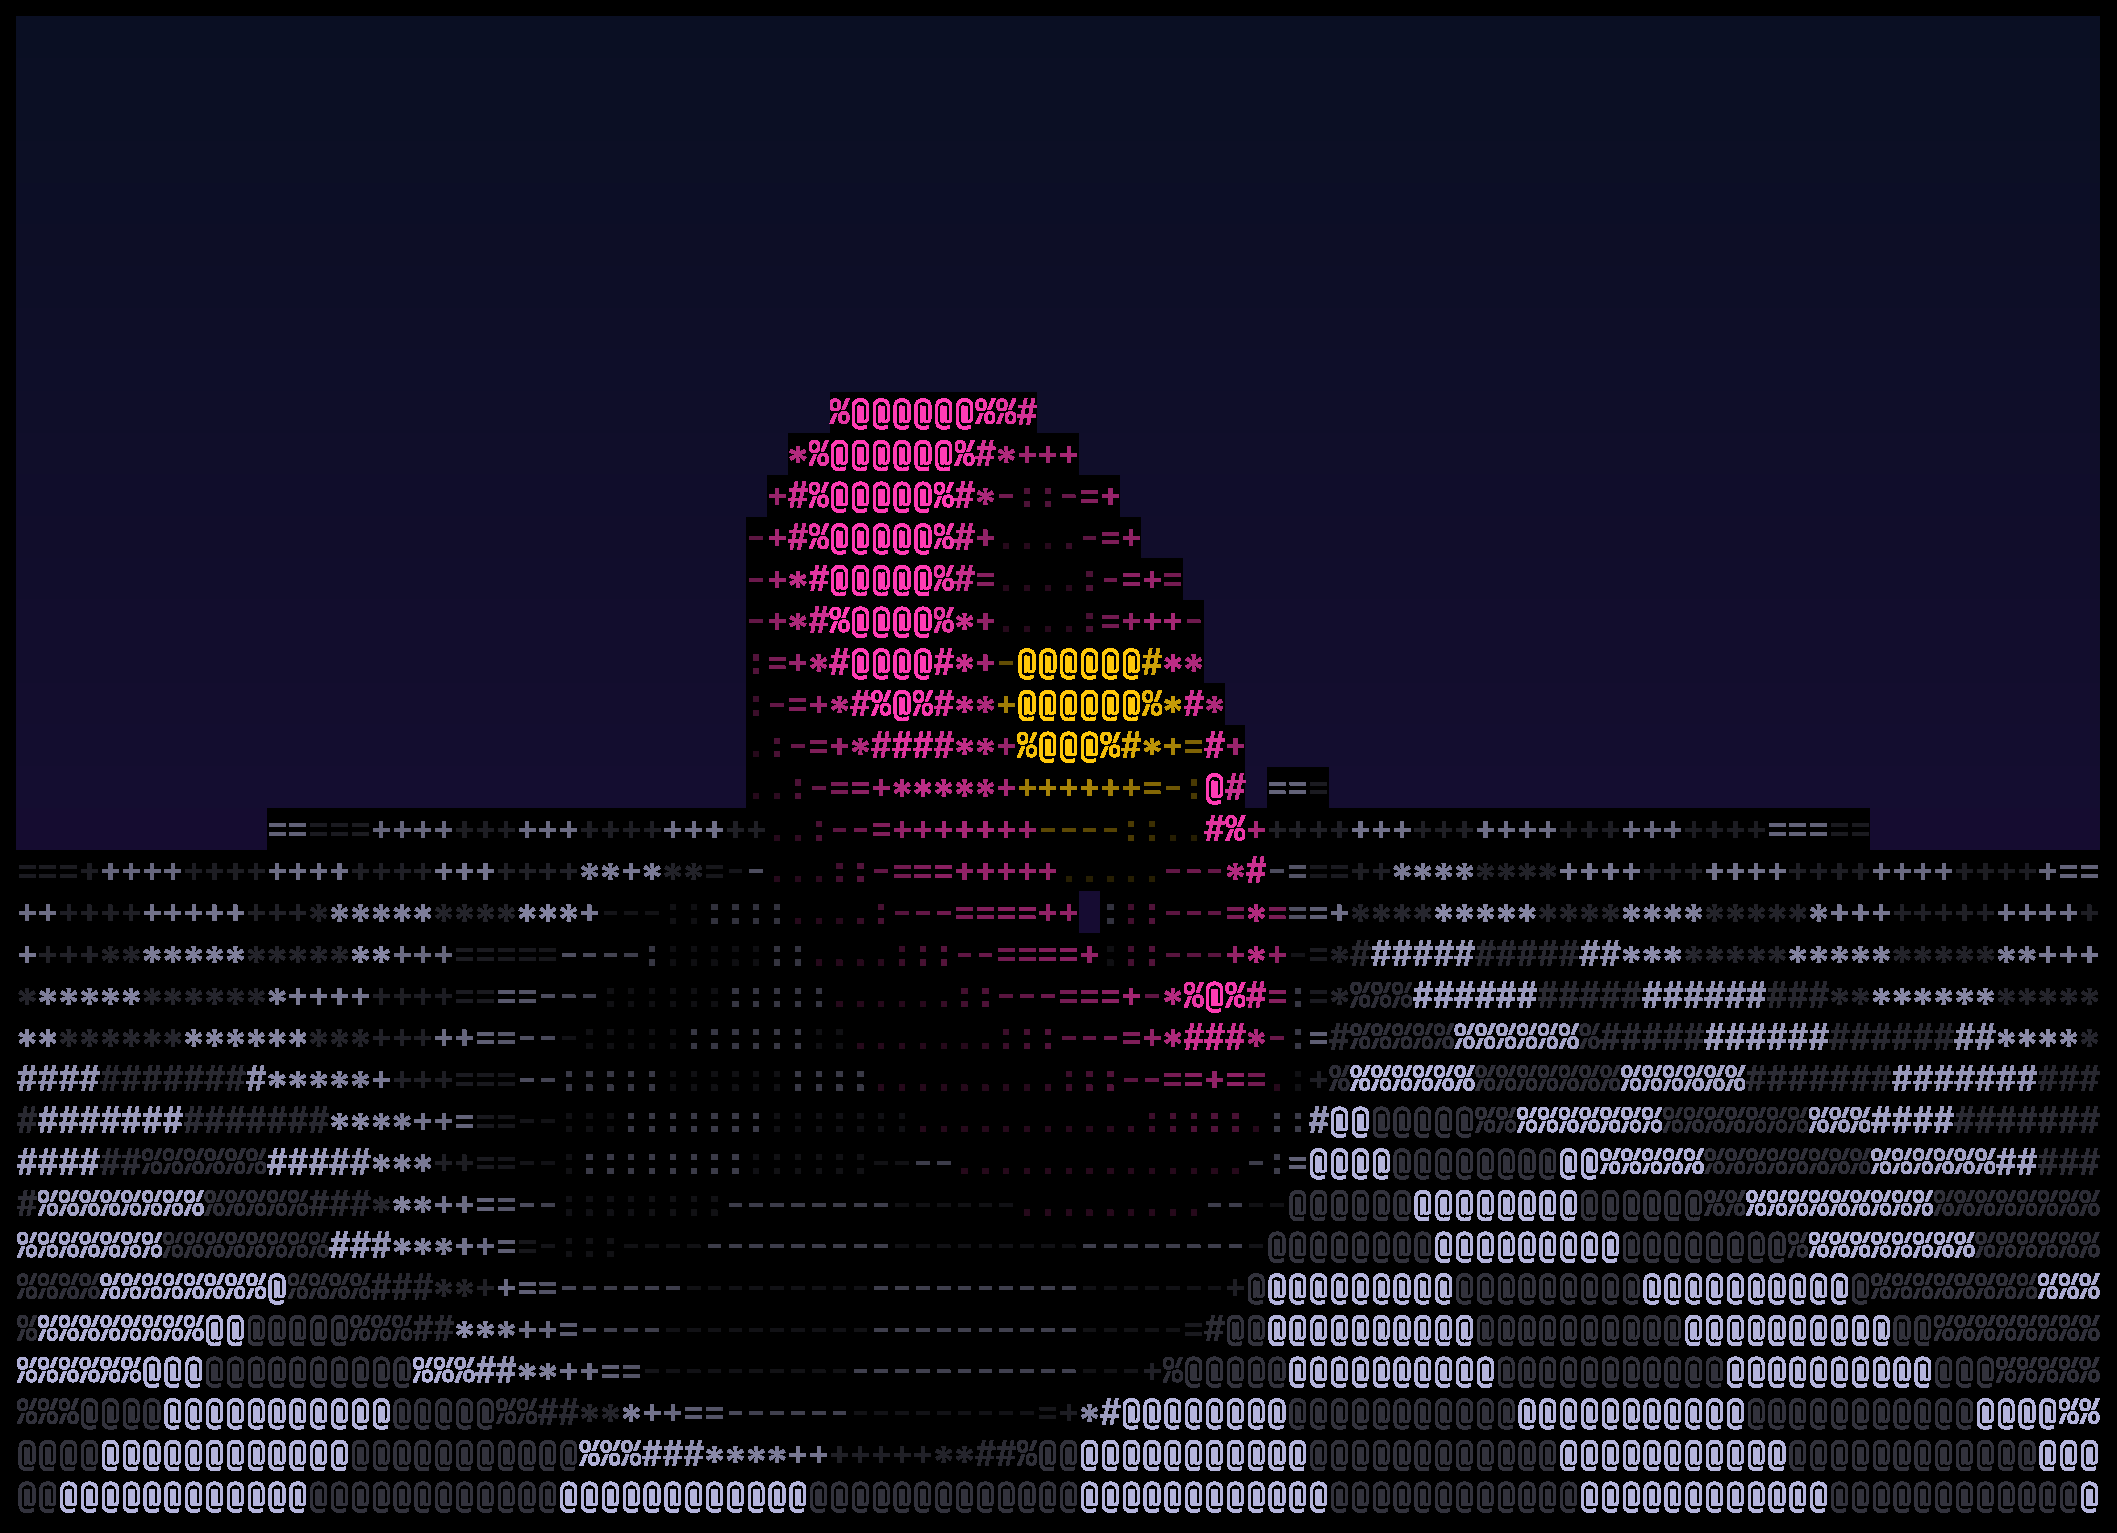
\includegraphics[width=\linewidth]{figures/demos/05-raymarching.pdf}

The raymarching example evaluates a signed-distance scene, estimates normals, combines lighting and shadows, then chooses an ASCII shading character and RGB values per cell. This is an actual Surface capture at 100 by 36 cells, frame 90 and elapsed time 1.5 seconds. The in-app control panel was disabled for the capture. Recursive Mono supplies the printed glyphs; the scene geometry and colors come from the demo.

\section{Metaballs and a denser subgrid}
\subsection{Sampling below a character cell}

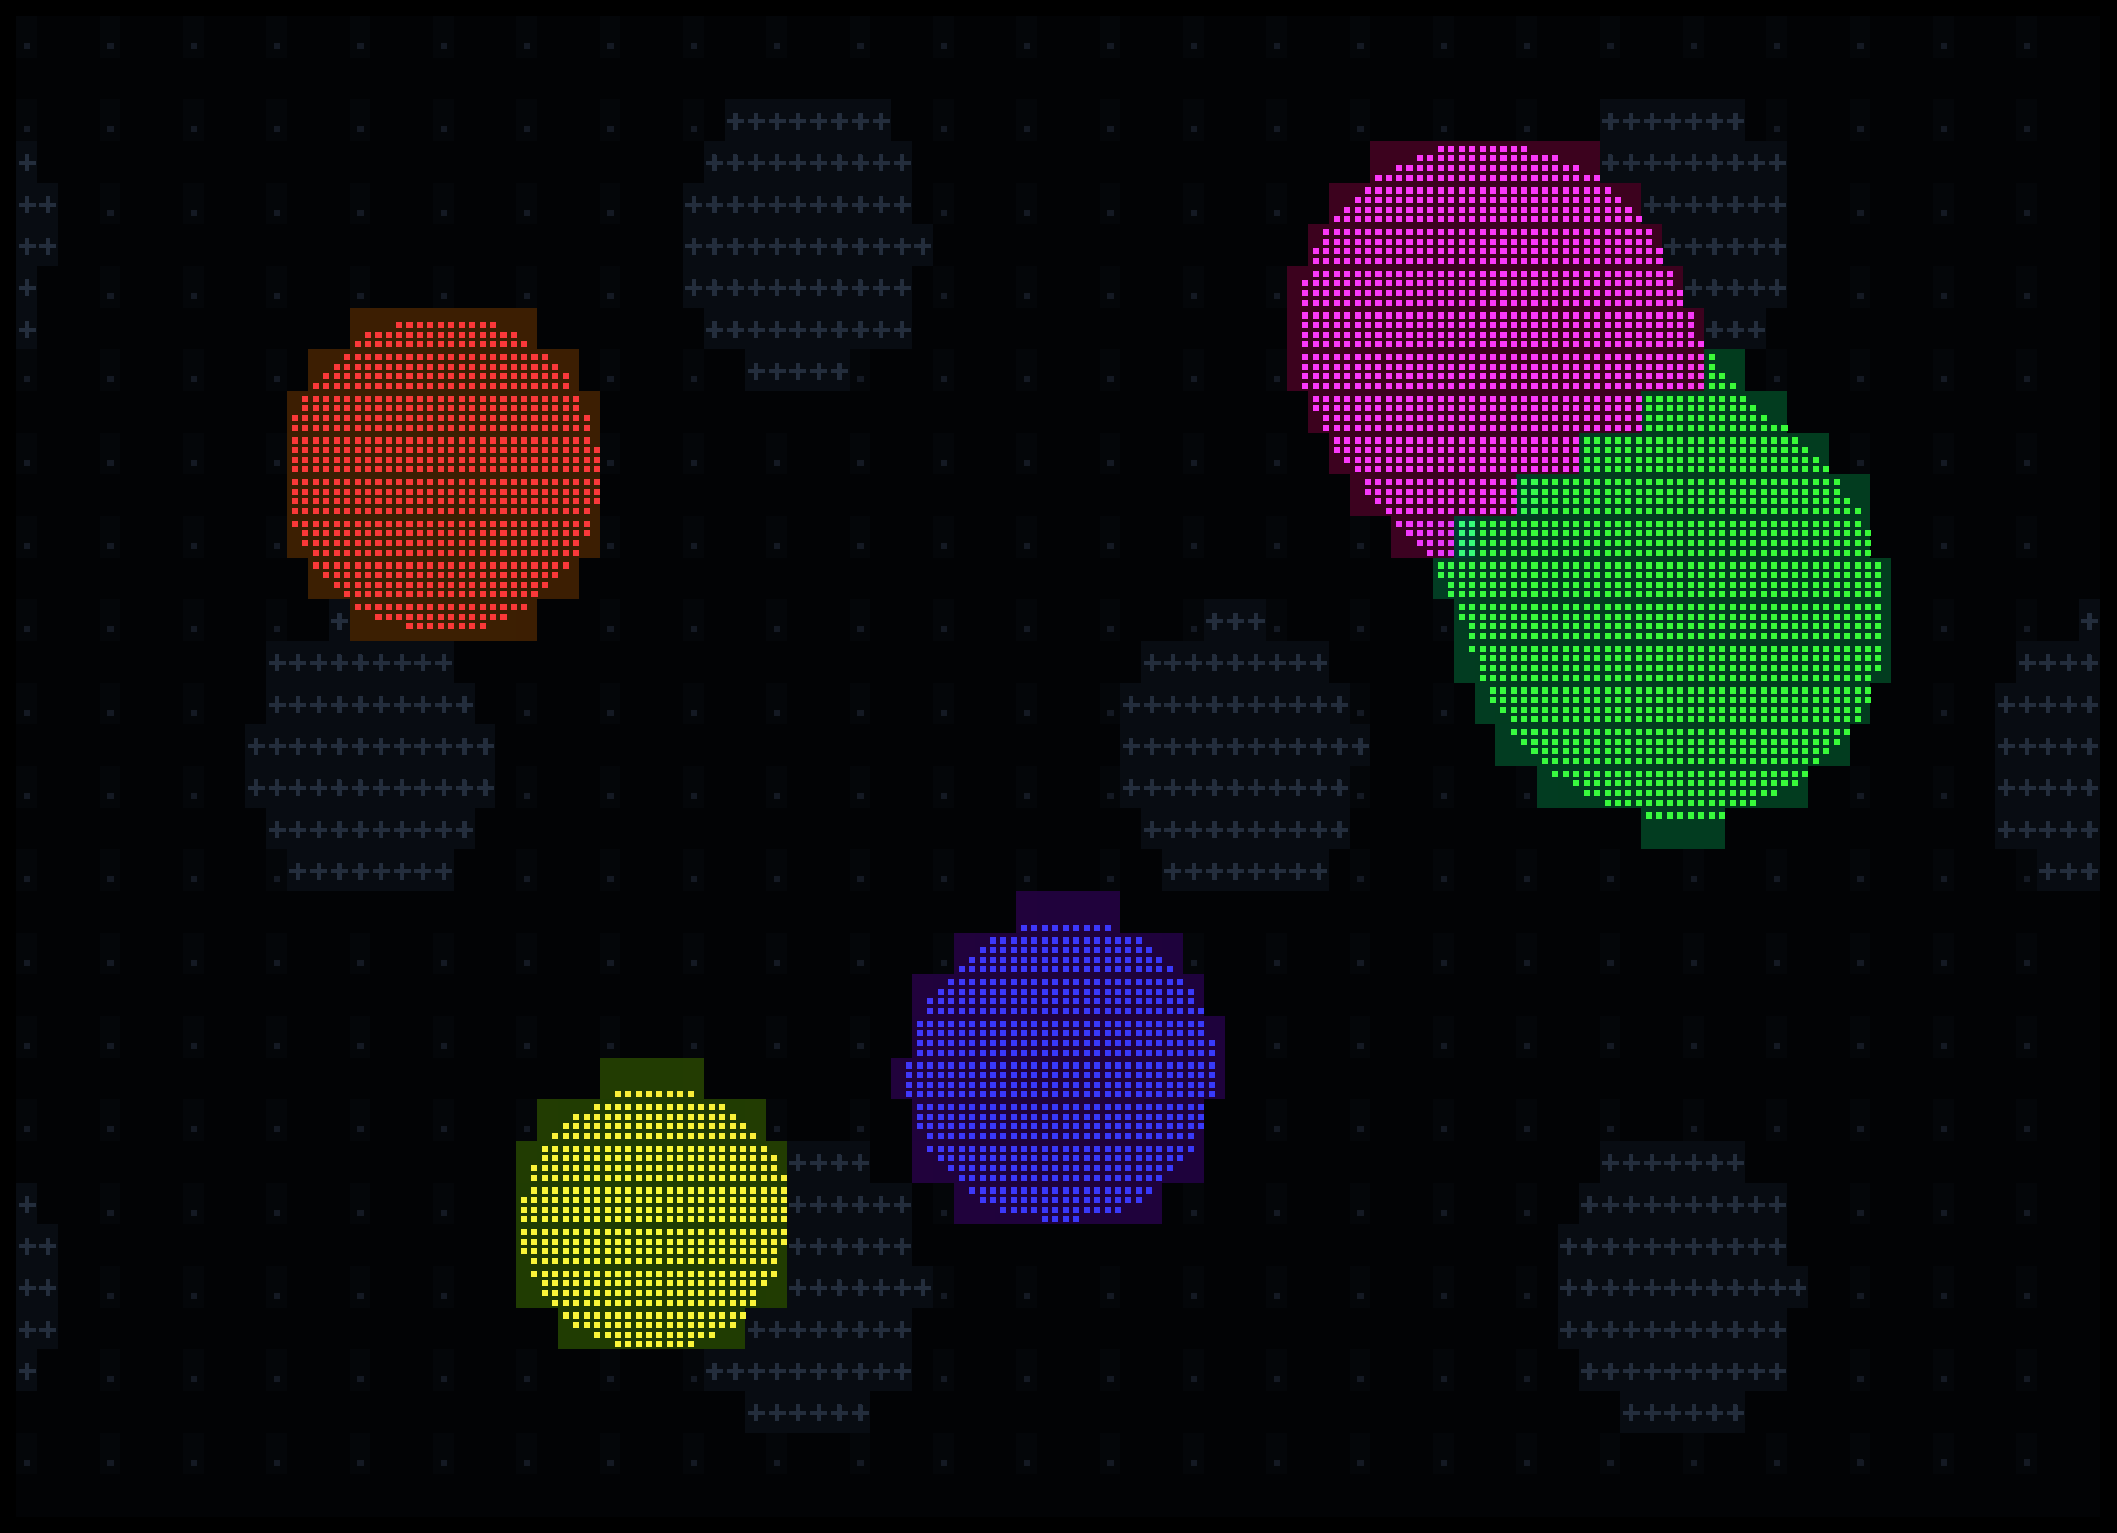
\includegraphics[width=\linewidth]{figures/demos/09-metaballs.pdf}

The metaballs example evaluates a binary subgrid with two samples across and four down for each terminal cell, then turns that pattern into a Braille character. It blends colors from the contributing fields. This capture uses the same viewport, frame and elapsed time, with the source's fixed default blob positions and the control panel hidden. DejaVu Sans supplies Braille symbols missing from Recursive.

\section{What an illustration establishes}
\subsection{A capture has a scope}

These figures show two deterministic rendered states. They do not establish frame rate, sustained resource use, interaction quality or cross-version compatibility. The source hashes, parameters and cell hashes are retained in \path{demo-manifest.json}. They are useful examples of how a renderer can make an image from terminal cells, alongside the more task-oriented job-monitor workshops.
